\documentclass[aspectratio=169]{beamer}
\usepackage[utf8]{inputenc}
\usepackage{tikz}
\usepackage{fontawesome5}
\usepackage{hyperref}
\usepackage{xcolor}
\usepackage{graphicx}
\usepackage{colortbl}
\usepackage{listings}

% Define Google Colors
\definecolor{googleblue}{RGB}{66, 133, 244}
\definecolor{googlered}{RGB}{234, 67, 53}
\definecolor{googleyellow}{RGB}{251, 188, 5}
\definecolor{googlegreen}{RGB}{52, 168, 83}
\definecolor{darkgrey}{RGB}{95, 99, 104}
\definecolor{lightgrey}{RGB}{241, 243, 244}

% Theme Settings
\usetheme{Madrid}
\usecolortheme[named=googleblue]{structure}

% Remove navigation symbols
\setbeamertemplate{navigation symbols}{}

% Header configuration
\setbeamertemplate{headline}{
    \leavevmode%
    \hbox{%
        \begin{beamercolorbox}[wd=.5\paperwidth,ht=2.5ex,dp=1ex,left]{section in head/foot}%
            \hspace{1em}\insertframenumber/\inserttotalframenumber\hspace{1em}
        \end{beamercolorbox}%
        \begin{beamercolorbox}[wd=.5\paperwidth,ht=2.5ex,dp=1ex,right]{subsection in head/foot}%
            \hspace{1em}\insertshorttitle\hspace{1em}
        \end{beamercolorbox}%
    }%
}

% Footer configuration with blue background and white text
\setbeamertemplate{footline}{
    \leavevmode%
    \hbox{%
        \begin{beamercolorbox}[wd=\paperwidth,ht=3ex,dp=1.5ex,center,colorbg=googleblue,colorfg=white]{footer}%
            \begin{minipage}{0.33\textwidth}
                \raggedright
                \hspace{1em}\href{https://easy-ai-labs.lovable.app/}{\color{white}Easy AI Labs}
            \end{minipage}%
            \begin{minipage}{0.33\textwidth}
                \centering
                \href{https://www.linkedin.com/in/yashkavaiya}{\color{white}Yash Kavaiya}
            \end{minipage}%
            \begin{minipage}{0.33\textwidth}
                \raggedleft
                \href{https://www.linkedin.com/company/genai-guru}{\color{white}Gen AI Guru}\hspace{1em}
            \end{minipage}
        \end{beamercolorbox}%
    }%
}

% Title and author information
\title[Conversational AI Resource Management]{Conversational AI Resource Management}
\subtitle{Complete Quiz Guide with Explanations}
\author{Presented by Yash Kavaiya}
\institute{Easy AI Labs \& Gen AI Guru}
\date{\today}

% Hyperref setup
\hypersetup{
    colorlinks=true,
    linkcolor=white,
    urlcolor=white,
    citecolor=white
}

\begin{document}

% Title Slide with Custom Design
\begin{frame}[plain]
    \begin{tikzpicture}[remember picture,overlay]
        % Background gradient
        \fill[googleblue] (current page.north west) rectangle (current page.south east);
        
        % Google colors accent bars
        \fill[googlered] ([yshift=-3cm]current page.north west) rectangle ++(0.5cm, -8cm);
        \fill[googleyellow] ([yshift=-3cm, xshift=0.6cm]current page.north west) rectangle ++(0.5cm, -8cm);
        \fill[googlegreen] ([yshift=-3cm, xshift=1.2cm]current page.north west) rectangle ++(0.5cm, -8cm);
        
        % Main content
        \node[white, font=\Huge\bfseries] at ([yshift=2cm]current page.center) {Conversational AI};
        \node[white, font=\LARGE] at ([yshift=0.5cm]current page.center) {Resource Management};
        \node[white, font=\large] at ([yshift=-0.8cm]current page.center) {Complete Quiz Guide};
        
        % Icon
        \node[white] at ([yshift=-2.5cm]current page.center) {\Huge\faRobot};
        
        % Author info
        \node[white, font=\normalsize] at ([yshift=-4.5cm]current page.center) {
            Presented by: Yash Kavaiya
        };
        \node[white, font=\small] at ([yshift=-5.5cm]current page.center) {
            Easy AI Labs | Gen AI Guru | \faCalendar\ \today
        };
    \end{tikzpicture}
\end{frame}

% Table of Contents
\begin{frame}{Today's Topics}
    \begin{columns}
        \column{0.5\textwidth}
        \begin{block}{\textcolor{googleblue}{\faClipboardList} Topics Covered}
            \begin{enumerate}
                \item Google Cloud DLP
                \item Conversational Agent Resources
                \item Project Association
                \item Best Practices
            \end{enumerate}
        \end{block}
        
        \column{0.5\textwidth}
        \begin{block}{\textcolor{googlegreen}{\faGraduationCap} Learning Objectives}
            \begin{itemize}
                \item Understand DLP functionality
                \item Learn resource deployment types
                \item Master project management
                \item Apply security best practices
            \end{itemize}
        \end{block}
    \end{columns}
    
    \vspace{1em}
    \begin{center}
        
\begin{tikzpicture}
            \draw[fill=googleyellow, draw=googleyellow] (0,0) rectangle (10,0.5);
            \node[darkgrey, font=\bfseries] at (5,0.25) {Let's test your knowledge!};
        \end{tikzpicture}
    \end{center}
\end{frame}

% Topic 1: Google Cloud DLP
\begin{frame}{Topic 1: Google Cloud Data Loss Prevention (DLP)}
    \begin{columns}
        \column{0.6\textwidth}
        \begin{block}{What is Google Cloud DLP?}
            \begin{itemize}
                \item Cloud-native data protection service
                \item Discovers and classifies sensitive data
                \item Provides de-identification and re-identification
                \item Helps meet compliance requirements
            \end{itemize}
        \end{block}
        
        \begin{block}{Key Features}
            \begin{itemize}
                \item[\textcolor{googlegreen}{\faCheck}] PII Detection
                \item[\textcolor{googlegreen}{\faCheck}] Data Redaction
                \item[\textcolor{googlegreen}{\faCheck}] Risk Analysis
                \item[\textcolor{googlegreen}{\faCheck}] Compliance Tools
            \end{itemize}
        \end{block}
        
        \column{0.4\textwidth}
        \begin{center}
            \begin{tikzpicture}
                \node[draw=googleblue, fill=lightgrey, rounded corners, minimum width=4cm, minimum height=3cm] {
                    \begin{minipage}{3.5cm}
                        \centering
                        \textcolor{googleblue}{\Huge\faShieldAlt}\\[0.5em]
                        \textbf{DLP}\\
                        Data Protection
                    \end{minipage}
                };
            \end{tikzpicture}
        \end{center}
    \end{columns}
\end{frame}

% Question 1 - Part 1: Question
\begin{frame}{Question 1: Google Cloud DLP Purpose}
    \begin{center}
        
\begin{tikzpicture}
            \node[draw=googleblue, fill=lightgrey, rounded corners, minimum width=12cm, minimum height=2cm, text=darkgrey, font=\Large\bfseries] {
                Google Cloud DLP is used to...?
            };
        \end{tikzpicture}
    \end{center}
    
    \vspace{1em}
    
    \begin{columns}
        \column{0.5\textwidth}
        \begin{block}{Option A}
            \textcolor{googlered}{\faTimesCircle} Redact information from voice recordings
        \end{block}
        
        \begin{block}{Option B}
            \textcolor{googlered}{\faTimesCircle} Make Conversational Agents perform better
        \end{block}
        
        \column{0.5\textwidth}
        \begin{block}{Option C}
            \textcolor{googlered}{\faTimesCircle} Generate synthetic data
        \end{block}
        
        \begin{block}{Option D}
            \textcolor{googlegreen}{\faCheckCircle} \textbf{Identify PII and redact where necessary}
        \end{block}
    \end{columns}
\end{frame}

% Question 1 - Part 2: Answer & Explanation
\begin{frame}{Question 1: Answer Explanation}
    \begin{alertblock}{Correct Answer: D - Identify PII and redact where necessary}
        \textcolor{googlegreen}{\faCheckCircle} This is the primary function of Google Cloud DLP
    \end{alertblock}
    
    \begin{block}{Why other options are incorrect:}
        \begin{itemize}
            \item[\textcolor{googlered}{\faTimes}] \textbf{Option A:} While DLP can work with text transcripts from voice, it doesn't directly process audio files
            \item[\textcolor{googlered}{\faTimes}] \textbf{Option B:} DLP focuses on data protection, not agent performance optimization
            \item[\textcolor{googlered}{\faTimes}] \textbf{Option C:} DLP is for protecting real data, not generating synthetic data
        \end{itemize}
    \end{block}
    
    \begin{exampleblock}{Real-world Application}
        DLP can detect and redact credit card numbers, social security numbers, email addresses, and other PII from documents, databases, and data streams in real-time.
    \end{exampleblock}
\end{frame}

% Topic 2: Conversational Agent Resources
\begin{frame}{Topic 2: Conversational Agent Resource Types}
    \begin{center}
        \begin{tikzpicture}
            % Global Resources
            \node[draw=googleblue, fill=googleblue!20, rounded corners, minimum width=5cm, minimum height=3cm] at (0,0) {
                \begin{minipage}{4.5cm}
                    \centering
                    \textcolor{googleblue}{\Large\faGlobe}\\[0.3em]
                    \textbf{Global Resources}\\[0.3em]
                    \small
                    • Available worldwide\\
                    • No region restrictions\\
                    • Automatic failover\\
                    • Higher availability
                \end{minipage}
            };
            
            % Regional Resources
            \node[draw=googlegreen, fill=googlegreen!20, rounded corners, minimum width=5cm, minimum height=3cm] at (6,0) {
                \begin{minipage}{4.5cm}
                    \centering
                    \textcolor{googlegreen}{\Large\faMapMarkerAlt}\\[0.3em]
                    \textbf{Regional Resources}\\[0.3em]
                    \small
                    • Specific location\\
                    • Data residency\\
                    • Lower latency\\
                    • Compliance needs
                \end{minipage}
            };
            
            % VS
            \node[draw=googleyellow, fill=googleyellow, text=white, circle, font=\bfseries] at (3,0) {VS};
        \end{tikzpicture}
    \end{center}
    
    \vspace{0.5em}
    
    \begin{block}{Key Consideration}
        Conversational Agents can be deployed as \textbf{either} global or regional resources based on your requirements
    \end{block}
\end{frame}

% Question 2 - Part 1: Question
\begin{frame}{Question 2: Agent Resource Types}
    \begin{center}
        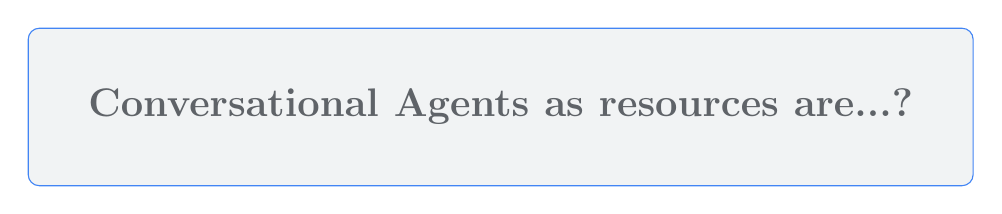
\begin{tikzpicture}
            \node[draw=googleblue, fill=lightgrey, rounded corners, minimum width=12cm, minimum height=2cm, text=darkgrey, font=\Large\bfseries] {
                Conversational Agents as resources are...?
            };
        \end{tikzpicture}
    \end{center}
    
    \vspace{1em}
    
    \begin{columns}
        \column{0.5\textwidth}
        \begin{block}{Option A}
            \textcolor{googlegreen}{\faCheckCircle} \textbf{Either global or regional}
        \end{block}
        
        \begin{block}{Option B}
            \textcolor{googlered}{\faTimesCircle} Neither global nor regional, they just work
        \end{block}
        
        \column{0.5\textwidth}
        \begin{block}{Option C}
            \textcolor{googlered}{\faTimesCircle} Only regional
        \end{block}
        
        \begin{block}{Option D}
            \textcolor{googlered}{\faTimesCircle} Only global
        \end{block}
    \end{columns}
\end{frame}

% Question 2 - Part 2: Answer & Explanation
\begin{frame}{Question 2: Answer Explanation}
    \begin{alertblock}{Correct Answer: A - Either global or regional}
        \textcolor{googlegreen}{\faCheckCircle} Conversational Agents offer flexibility in deployment scope
    \end{alertblock}
    
    \begin{columns}
        \column{0.5\textwidth}
        \begin{block}{When to use Global}
            \begin{itemize}
                \item Multi-region applications
                \item High availability needs
                \item Global user base
                \item Disaster recovery
            \end{itemize}
        \end{block}
        
        \column{0.5\textwidth}
        \begin{block}{When to use Regional}
            \begin{itemize}
                \item Data sovereignty laws
                \item GDPR compliance
                \item Low latency requirements
                \item Cost optimization
            \end{itemize}
        \end{block}
    \end{columns}
    
    \vspace{0.5em}
    
    \begin{exampleblock}{Best Practice}
        Choose deployment type based on your compliance requirements, user location, and performance needs.
    \end{exampleblock}
\end{frame}

% Topic 3: Project Association
\begin{frame}{Topic 3: Google Cloud Project Association}
    \begin{block}{Project-Based Organization}
        All Google Cloud resources, including Conversational Agents, are organized within projects
    \end{block}
    
    \begin{columns}
        \column{0.33\textwidth}
        \begin{center}
            \textcolor{googleblue}{\Huge\faFolder}\\
            \textbf{Organization}\\
            \small Top-level container
        \end{center}
        
        \column{0.33\textwidth}
        \begin{center}
            \textcolor{googleyellow}{\Huge\faProjectDiagram}\\
            \textbf{Project}\\
            \small Resource container
        \end{center}
        
        \column{0.33\textwidth}
        \begin{center}
            \textcolor{googlegreen}{\Huge\faRobot}\\
            \textbf{Agent}\\
            \small Your resource
        \end{center}
    \end{columns}
    
    \vspace{1em}
    
    \begin{block}{Benefits of Project Association}
        \begin{itemize}
            \item[\textcolor{googlegreen}{\faCheck}] Centralized billing and cost tracking
            \item[\textcolor{googlegreen}{\faCheck}] IAM access control and permissions
            \item[\textcolor{googlegreen}{\faCheck}] Resource isolation and organization
            \item[\textcolor{googlegreen}{\faCheck}] Quota and limit management
        \end{itemize}
    \end{block}
\end{frame}

% Question 3 - Part 1: Question
\begin{frame}{Question 3: Agent Creation}
    \begin{center}
        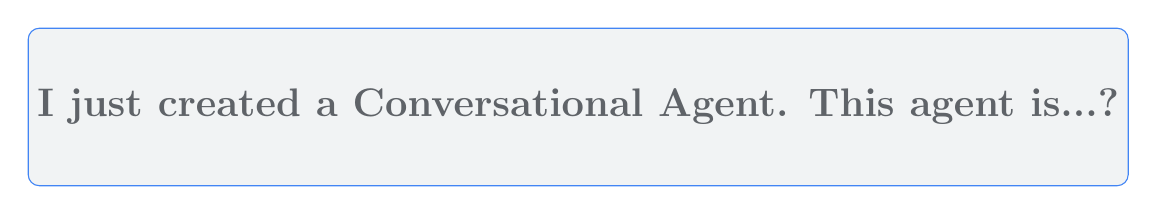
\begin{tikzpicture}
            \node[draw=googleblue, fill=lightgrey, rounded corners, minimum width=12cm, minimum height=2cm, text=darkgrey, font=\Large\bfseries] {
                I just created a Conversational Agent. This agent is...?
            };
        \end{tikzpicture}
    \end{center}
    
    \vspace{1em}
    
    \begin{columns}
        \column{0.5\textwidth}
        \begin{block}{Option A}
            \textcolor{googlegreen}{\faCheckCircle} \textbf{Associated with a Google Cloud project}
        \end{block}
        
        \begin{block}{Option B}
            \textcolor{googlered}{\faTimesCircle} Managed in Google Cloud Folders
        \end{block}
        
        \column{0.5\textwidth}
        \begin{block}{Option C}
            \textcolor{googlered}{\faTimesCircle} Not associated with any Google Cloud resources
        \end{block}
        
        \begin{block}{Option D}
            \textcolor{googlered}{\faTimesCircle} Available from any Google Cloud project
        \end{block}
    \end{columns}
\end{frame}

% Question 3 - Part 2: Answer & Explanation
\begin{frame}{Question 3: Answer Explanation}
    \begin{alertblock}{Correct Answer: A - Associated with a Google Cloud project}
        \textcolor{googlegreen}{\faCheckCircle} Every Conversational Agent must belong to a specific project
    \end{alertblock}
    
    \begin{block}{Why Project Association is Important}
        \begin{itemize}
            \item \textbf{Resource Management:} Organize and track all related resources
            \item \textbf{Access Control:} Use IAM to manage who can access the agent
            \item \textbf{Billing:} Track costs at the project level
            \item \textbf{Quotas:} Apply project-specific limits and quotas
        \end{itemize}
    \end{block}
    
    \begin{columns}
        \column{0.5\textwidth}
        \begin{exampleblock}{Example Structure}
            \small
            \texttt{Organization/}\\
            \texttt{├── Project-Dev/}\\
            \texttt{│   └── Agent-Test}\\
            \texttt{└── Project-Prod/}\\
            \texttt{    └── Agent-Live}
        \end{exampleblock}
        
        \column{0.5\textwidth}
        \begin{block}{Note}
            Agents are \textbf{NOT}:
            \begin{itemize}
                \item Shared across projects
                \item Managed at folder level
                \item Independent resources
            \end{itemize}
        \end{block}
    \end{columns}
\end{frame}

% Summary of All Questions
\begin{frame}{Quiz Summary}
    \begin{center}
        \textbf{\Large All Questions at a Glance}
    \end{center}
    
    \vspace{0.5em}
    
    \begin{tikzpicture}
        % Question 1
        \node[draw=googleblue, fill=googleblue!20, rounded corners, minimum width=13cm, minimum height=1.8cm] at (0,3) {
            \begin{minipage}{12cm}
                \textbf{Q1: Google Cloud DLP Purpose}\\
                \textcolor{googlegreen}{\faCheckCircle} Identify PII and redact where necessary
            \end{minipage}
        };
        
        % Question 2
        \node[draw=googleyellow, fill=googleyellow!20, rounded corners, minimum width=13cm, minimum height=1.8cm] at (0,1) {
            \begin{minipage}{12cm}
                \textbf{Q2: Agent Resource Types}\\
                \textcolor{googlegreen}{\faCheckCircle} Either global or regional
            \end{minipage}
        };
        
        % Question 3
        \node[draw=googlegreen, fill=googlegreen!20, rounded corners, minimum width=13cm, minimum height=1.8cm] at (0,-1) {
            \begin{minipage}{12cm}
                \textbf{Q3: Agent Project Association}\\
                \textcolor{googlegreen}{\faCheckCircle} Associated with a Google Cloud project
            \end{minipage}
        };
        
        % Score
        \node[draw=googlered, fill=googlered, text=white, rounded corners, minimum width=4cm, minimum height=1cm, font=\bfseries] at (0,-3) {
            Perfect Score: 100\%
        };
    \end{tikzpicture}
\end{frame}

% Best Practices Deep Dive
\begin{frame}{Best Practices for Implementation}
    \begin{columns}
        \column{0.5\textwidth}
        \begin{block}{\textcolor{googleblue}{\faShieldAlt} Security Best Practices}
            \begin{itemize}
                \item Enable DLP for all text inputs
                \item Regular security audits
                \item Implement least privilege access
                \item Monitor API usage patterns
            \end{itemize}
        \end{block}
        
        \begin{block}{\textcolor{googlegreen}{\faCogs} Operational Excellence}
            \begin{itemize}
                \item Use version control for agents
                \item Implement CI/CD pipelines
                \item Regular backup strategies
                \item Performance monitoring
            \end{itemize}
        \end{block}
        
        \column{0.5\textwidth}
        \begin{block}{\textcolor{googleyellow}{\faChartLine} Performance Optimization}
            \begin{itemize}
                \item Choose appropriate regions
                \item Implement caching strategies
                \item Optimize conversation flows
                \item Load balancing for high traffic
            \end{itemize}
        \end{block}
        
        \begin{block}{\textcolor{googlered}{\faDollarSign} Cost Management}
            \begin{itemize}
                \item Set up billing alerts
                \item Use committed use discounts
                \item Regular resource cleanup
                \item Monitor usage patterns
            \end{itemize}
        \end{block}
    \end{columns}
\end{frame}

% Common Pitfalls
\begin{frame}{Common Pitfalls to Avoid}
    \begin{enumerate}
        \item[\textcolor{googlered}{\faBan}] \textbf{Not enabling DLP}
        \begin{itemize}
            \item Risk of exposing sensitive data
            \item Compliance violations
        \end{itemize}
        
        \item[\textcolor{googlered}{\faBan}] \textbf{Wrong resource scope selection}
        \begin{itemize}
            \item Choosing global when regional is required for compliance
            \item Missing latency requirements
        \end{itemize}
        
        \item[\textcolor{googlered}{\faBan}] \textbf{Poor project organization}
        \begin{itemize}
            \item Mixing dev and production resources
            \item No clear naming conventions
        \end{itemize}
        
        \item[\textcolor{googlered}{\faBan}] \textbf{Inadequate access control}
        \begin{itemize}
            \item Over-permissive IAM roles
            \item No service account management
        \end{itemize}
    \end{enumerate}
    
    \begin{center}
        
\begin{tikzpicture}
            \draw[fill=googleyellow, draw=googleyellow] (0,0) rectangle (8,0.5);
            \node[darkgrey, font=\bfseries] at (4,0.25) {Avoid these for successful deployment!};
        \end{tikzpicture}
    \end{center}
\end{frame}

% Additional Resources
\begin{frame}{Additional Learning Resources}
    \begin{columns}
        \column{0.5\textwidth}
        \begin{block}{\textcolor{googleblue}{\faBook} Documentation}
            \begin{itemize}
                \item Google Cloud DLP Docs
                \item Dialogflow CX Guide
                \item Best Practices Guide
                \item API References
            \end{itemize}
        \end{block}
        
        \begin{block}{\textcolor{googlegreen}{\faGraduationCap} Training}
            \begin{itemize}
                \item Google Cloud Skills Boost
                \item Coursera Specializations
                \item YouTube Tutorials
                \item Hands-on Labs
            \end{itemize}
        \end{block}
        
        \column{0.5\textwidth}
        \begin{block}{\textcolor{googleyellow}{\faUsers} Community}
            \begin{itemize}
                \item Stack Overflow
                \item Google Cloud Community
                \item Reddit r/googlecloud
                \item LinkedIn Groups
            \end{itemize}
        \end{block}
        
        \begin{block}{\textcolor{googlered}{\faCertificate} Certifications}
            \begin{itemize}
                \item Professional Cloud Architect
                \item Professional ML Engineer
                \item Associate Cloud Engineer
                \item Professional Cloud Developer
            \end{itemize}
        \end{block}
    \end{columns}
\end{frame}

% Key Takeaways
\begin{frame}{Key Takeaways}
    \begin{center}
        \textbf{\Large Remember These Core Concepts}
    \end{center}
    
    \vspace{1em}
    
    \begin{columns}
        \column{0.33\textwidth}
        \begin{center}
            \begin{tikzpicture}
                \node[draw=googleblue, fill=googleblue!20, circle, minimum width=3cm, minimum height=3cm] {
                    \begin{minipage}{2.5cm}
                        \centering
                        \textcolor{googleblue}{\Large\faShieldAlt}\\[0.3em]
                        \textbf{DLP}\\
                        \small Protects PII
                    \end{minipage}
                };
            \end{tikzpicture}
        \end{center}
        
        \column{0.33\textwidth}
        \begin{center}
            \begin{tikzpicture}
                \node[draw=googleyellow, fill=googleyellow!20, circle, minimum width=3cm, minimum height=3cm] {
                    \begin{minipage}{2.5cm}
                        \centering
                        \textcolor{googleyellow}{\Large\faGlobe}\\[0.3em]
                        \textbf{Flexible}\\
                        \small Global/Regional
                    \end{minipage}
                };
            \end{tikzpicture}
        \end{center}
        
        \column{0.33\textwidth}
        \begin{center}
            \begin{tikzpicture}
                \node[draw=googlegreen, fill=googlegreen!20, circle, minimum width=3cm, minimum height=3cm] {
                    \begin{minipage}{2.5cm}
                        \centering
                        \textcolor{googlegreen}{\Large\faProjectDiagram}\\[0.3em]
                        \textbf{Organized}\\
                        \small Project-based
                    \end{minipage}
                };
            \end{tikzpicture}
        \end{center}
    \end{columns}
    
    \vspace{1em}
    
    \begin{alertblock}{Success Formula}
        \centering
        \textbf{Security + Right Deployment + Good Organization = Successful AI Implementation}
    \end{alertblock}
\end{frame}

% Follow for More Updates - Final Slide
\begin{frame}[plain]
    \begin{tikzpicture}[remember picture,overlay]
        % Background
        \fill[googleblue] (current page.north west) rectangle (current page.south east);
        
        % Title
        \node[white, font=\Huge\bfseries] at ([yshift=3cm]current page.center) {
            Follow for More Updates!
        };
        
        % Content Details
        \node[white, font=\large] at ([yshift=1.5cm]current page.center) {
            \faInfoCircle\ Stay Connected for Latest AI Insights
        };
        
        % Social Links
        \node[draw=white, fill=white, fill opacity=0.1, rounded corners, minimum width=12cm, minimum height=1.5cm] at ([yshift=-0.5cm]current page.center) {
            \begin{minipage}{11cm}
                \centering
                \textcolor{white}{\Large\faLinkedin\ LinkedIn Profiles}\\[0.3em]
                \href{https://www.linkedin.com/in/yashkavaiya}{\textcolor{white}{\textbf{Yash Kavaiya} - AI Expert \& Educator}}\\
                \href{https://www.linkedin.com/company/genai-guru}{\textcolor{white}{\textbf{Gen AI Guru} - AI Community}}
            \end{minipage}
        };
        
        \node[draw=white, fill=white, fill opacity=0.1, rounded corners, minimum width=12cm, minimum height=1.5cm] at ([yshift=-2.5cm]current page.center) {
            \begin{minipage}{11cm}
                \centering
                \textcolor{white}{\Large\faYoutube\ YouTube Channel}\\[0.3em]
                \href{https://www.youtube.com/@YashKavaiya}{\textcolor{white}{\textbf{Subscribe for Weekly AI Tutorials}}}\\
                \textcolor{white}{\small New videos every week on AI, ML, and Cloud Technologies}
            \end{minipage}
        };
        
        \node[draw=white, fill=white, fill opacity=0.1, rounded corners, minimum width=12cm, minimum height=1.5cm] at ([yshift=-4.5cm]current page.center) {
            \begin{minipage}{11cm}
                \centering
                \textcolor{white}{\Large\faLaptopCode\ Easy AI Labs}\\[0.3em]
                \href{https://easy-ai-labs.lovable.app/}{\textcolor{white}{\textbf{Visit Our Platform}}}\\
                \textcolor{white}{\small Hands-on AI Labs and Projects}
            \end{minipage}
        };
        
        % Bottom message
        \node[white, font=\normalsize\bfseries] at ([yshift=-6cm]current page.center) {
            \faHeart\ Thank you for learning with us! Keep exploring AI! \faHeart
        };
    \end{tikzpicture}
\end{frame}

\end{document}